\subsection{Results}

\noindent If the treatment affects health outcomes, it does so by impacting the incidence rate of health conditions. For an individual, health conditions in turn impact their medical costs and quality of life. It is worth noting that lifetime medical costs depend on the severity of health events, however, they also depend on length of life in two ways: individuals who live longer accumulate medical costs over more years and medical costs increase with age. Because of this, it is important to quantify the benefits of an extra year of life that is healthy. Therefore, we look at the treatment effects on both medical costs and QALYs. \\


%Table~\ref{table:prevalence65} shows the prevalence of six chronic conditions between ages 40 and 65, when chronic conditions and diseases are majorly developed.\footnote{There are also differences in government transfer program participation rates. For example, 14\% of males in the treatment group are expected to claim disability insurance by age 60, while the males in the control group are expected to have a higher claiming rate of 25\%. The treatment effect for females at age 60 is much lower, showing only a 4\% difference.} \\
%In future work, we will monetize the treatment effect in program participation as well.

%\begin{table}[H]
%\begin{threeparttable}
%\footnotesize
%\caption{Prevalence of Disease from Ages 40 to 65} \label{table:prevalence65}
%\begin{tabular}{lcccc} \toprule
 & \multicolumn{2}{c}{Female} & \multicolumn{2}{c}{Female} \\
 & Control  & Treatment  & Control  & Treatment  \\  \midrule 
Cancer              &     0.198 &     0.131 &     0.000 &     0.036 \\  
Diabetes           &     0.319 &     0.298 &     0.129 &     0.366 \\  
Heart Diseases  &     0.158 &     0.211 &     0.110 &     0.105 \\  
Hypertension    &     0.816 &     0.813 &     0.484 &     0.631 \\  
Lunge Disease  &     0.172 &     0.228 &     0.187 &     0.095 \\  
Stroke Disease &     0.098 &     0.062 &     0.071 &     0.036 \\  \toprule \end{tabular}

%\begin{tablenotes}
%\footnotesize
%\item Note: Prevalence of six chronic conditions in the microsimulation exercise for the treatment and control groups by age 65, and by gender.
%\end{tablenotes}
%\end{threeparttable}
%\end{table}

\noindent The projections for health outcomes of treatment and control groups differ in the prevalence of chronic conditions. These differences in prevalence of health conditions impact medical costs and QALYs for these groups. Figures~\ref{figure:qaly} and~\ref{figure:totmd} show the evolution from age 30 of average QALYs and medical costs from all sources over the simulated life-cycle of the treatment and control groups.\footnote{This measure of total costs combines medical spending paid by private health insurance, public insurance, spending paid out-of-pocket, and all other sources.} 
%The averages shown are not conditional on survival, hence they drop to zero when everyone in the cohort is projected to have died.

\begin{figure}[H]
    \centering
\caption{Predicted Quality-Adjusted Life Years} \label{figure:qaly}
\begin{subfigure}{.8\textwidth}
  \centering
  \subcaption{Males}
  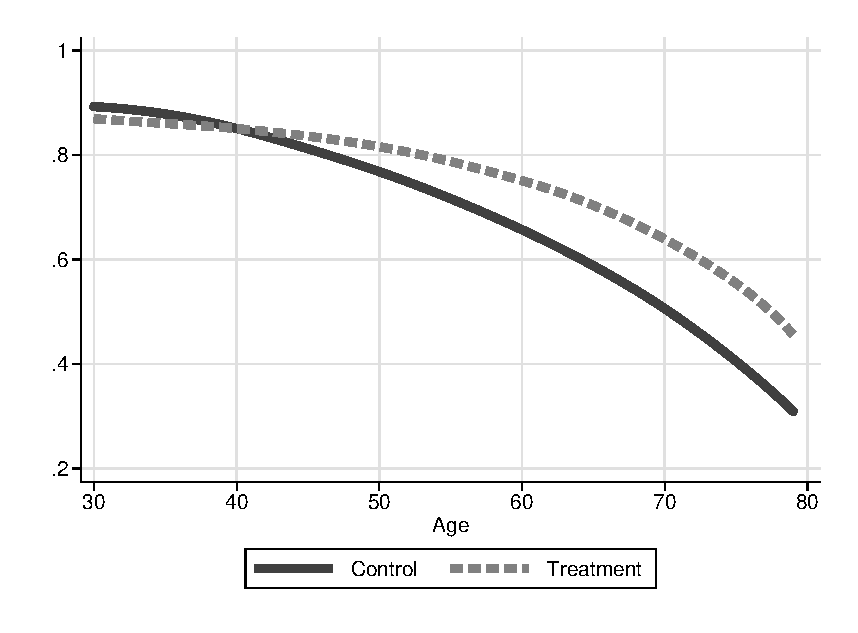
\includegraphics[height=3.5in]{AppOutput/Health/ABC-FAM_qaly_surv_summary_male}
\end{subfigure}

\begin{subfigure}{.8\textwidth} %
  \centering
  \subcaption{Females}
  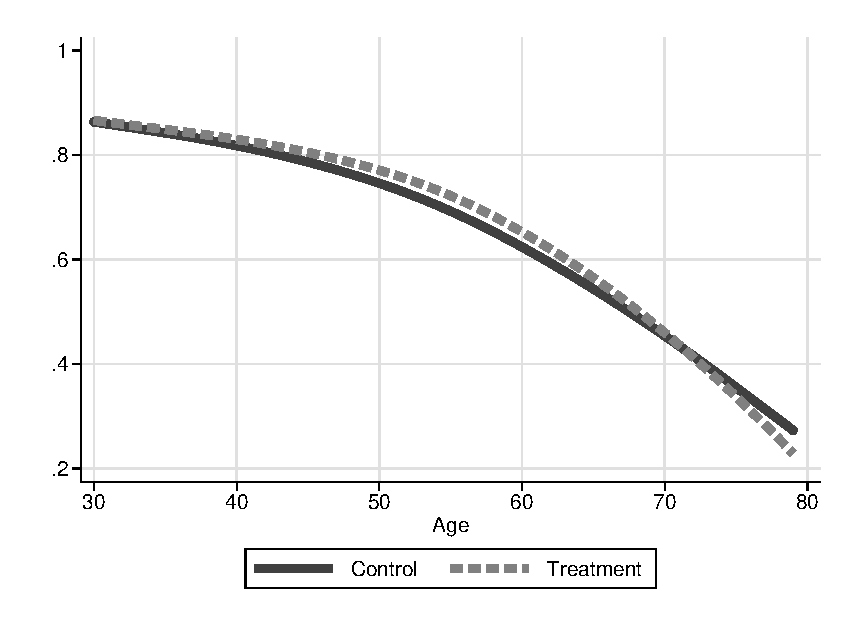
\includegraphics[height=3.5in]{AppOutput/Health/ABC-FAM_qaly_surv_summary_female}
\end{subfigure}
\floatfoot{
\footnotesize
\noindent Note: Panel (a) displays the predicted Quality-Adjusted Life Years (QALYs) from age 30 for males. Panel (b) displays the predicted Quality-Adjusted Life Years (QALYs) from age 30 for females.
}
\end{figure}
\begin{figure}[H]
    \centering
\caption{Predicted Total Medical Costs} \label{figure:totmd}
\begin{subfigure}{.8\textwidth}
  \centering
  \subcaption{Males}
  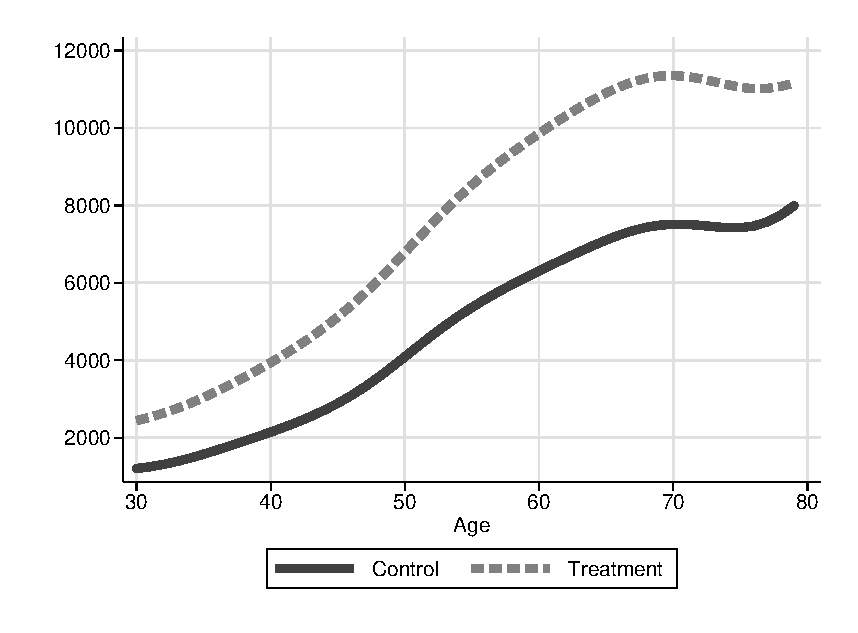
\includegraphics[height=3.5in]{AppOutput/Health/ABC-FAM_totmd_surv_summary_male}
\end{subfigure}

\begin{subfigure}{.8\textwidth} %
  \centering
  \subcaption{Females}
  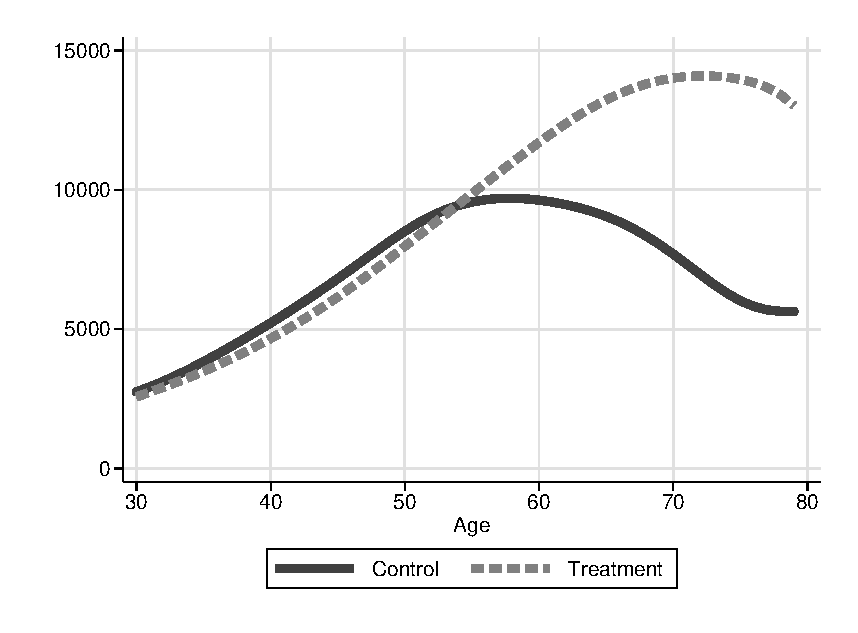
\includegraphics[height=3.5in]{AppOutput/Health/ABC-FAM_totmd_surv_summary_female}
\end{subfigure}
\floatfoot{
\footnotesize
\noindent Note: Panel (a) displays the predicted total medical costs for males over the life cycle from age 30 in 2009 USD. Panel (b) displays the predicted total medical costs for females over the life-cycle from age 30 in 2009 USD.
}
\end{figure}

\noindent Figure~\ref{figure:qaly} shows that predicted QALYs are higher over the entire life cycle for the treatment group than for the control group. This difference appears to be larger for males. This is not surprising, given that males show larger treatment effects in prevalence rates of disease than do females. Similarly, projected total medical costs are lower for the treatment group than for the control group over the entire life-cycle, as shown in Figure~\ref{figure:totmd}.
Figure~\ref{figure:fam_survival} shows estimates of the survival probability for the treatment and control groups in FAM. There is a substantial difference in survival rates in favor of males in the treatment groups when compared with those in the control groups. \\


\begin{figure}[H]
    \centering
\caption{Predicted Survival} \label{figure:fam_survival}
\begin{subfigure}{.8\textwidth}
  \centering
  \subcaption{Males}
  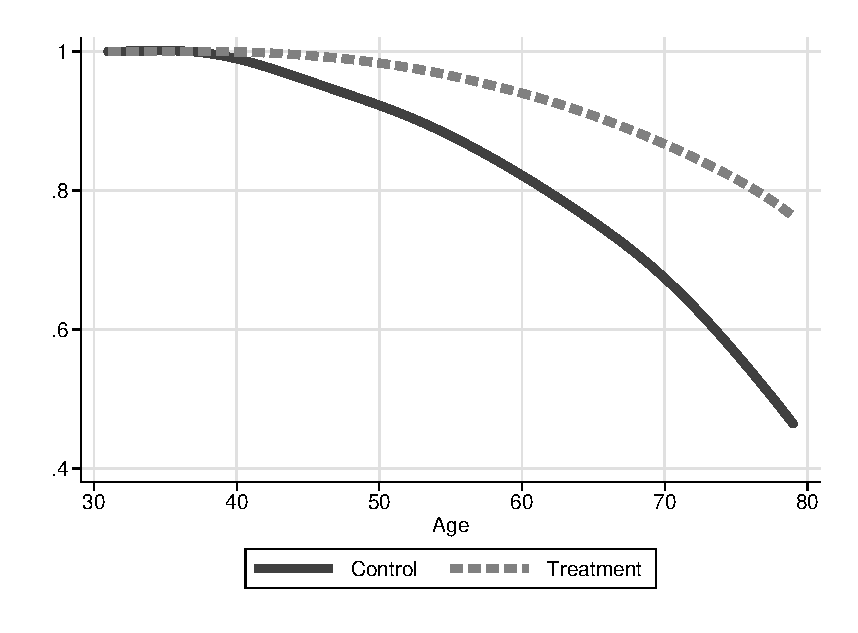
\includegraphics[height=3.5in]{AppOutput/Health/ABC-FAM_survival_male}
\end{subfigure}

\begin{subfigure}{.8\textwidth} %
  \centering
  \subcaption{Females}
  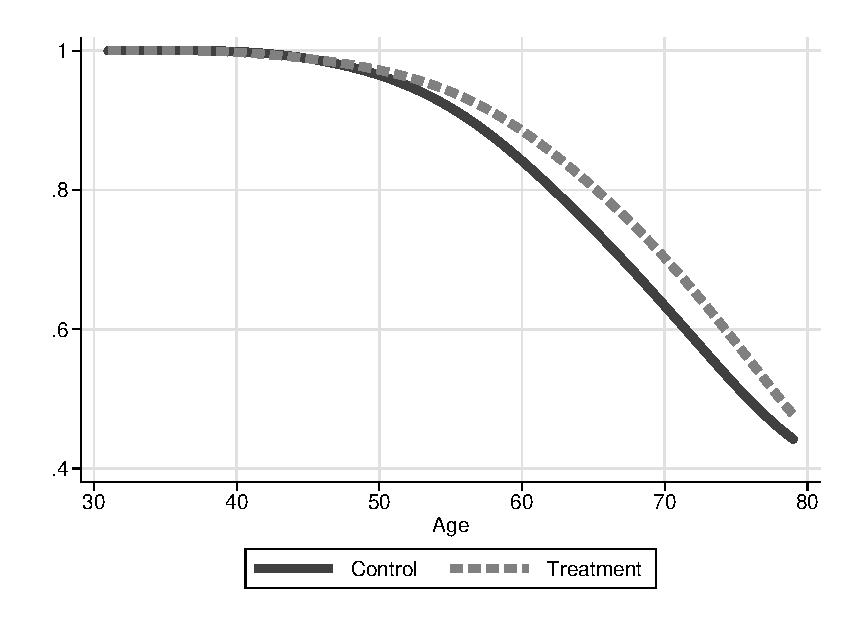
\includegraphics[height=3.5in]{AppOutput/Health/ABC-FAM_survival_female}
\end{subfigure}
\floatfoot{
\footnotesize
\noindent Note 1 Panel (a) displays the predicted survival for males after age-30 interview. Panel (b) displays the predicted survival for females after age-30 interview. Individual-level survival probabilities are calculated by estimating age-specific mortality probabilities for each subject using the FAM simulation results.  The individual-level survival probabilities are then averaged over the number of subjects in each group who had completed the age 34 interview.
}
\end{figure}

\noindent To quantify the impact of treatment on health outcomes, for each simulated cohort, we compute the present discounted value of the difference between treatment and control in the average value of QALYs and average medical costs. We do this for every age. We assume a discount rate of 4\% for this analysis, and we include outcome averages from the start of the simulation at age 30 until death for each cohort. We follow the recent literature on benefit-cost analysis of medical interventions and value a QALY of 1 to be worth \$150,000.\footnote{For a discussion on the limitations of a single value per QALY, see \citet{Pinto-Prades_etal_2009_Trying-to-Estimate} and \citet{Mason_etal_2009_Modelling}. \citet{Grosse_2008_Assessing-Cost-Effectiveness} summarizes the history of QALY valuation.} The raw difference in present discounted value at birth between treatment and control groups amounts to $ \$37,316  $ (2014 USD) per individual. Accounting for attrition, this difference falls to $ \$19,985 $. Table~\ref{table:PDV} shows the present discounted value of health outcomes for treatment and control cohorts in the top panel. The bottom panel of Table~\ref{table:PDV} decomposes the treatment effects on health by gender. The difference in health by treatment group is larger for males than for females. To account for a lack of consensus on QALY valuation, we also present the results for a lower valuation of QALYs, following \citet{Cutler_Meara_1998_Med-Costs_BOOK}, in the second row of each panel of Table~\ref{table:PDV}.\footnote{In Appendix \ref{appendix:sensitivity}, we show how the internal rate of return and benefit-cost ratios are impacted by a range of valuations for QALYs.} In this case of lower valuation of QALYs, there is still a positive difference in net health outcomes in favor of the treatment groups over the control groups of $ \$26,374$. Accounting for attrition, this difference falls to $ \$13,323$. \\

\begin{table}[H]
\begin{threeparttable}
%\footnotesize
\small
\caption{Present Discounted Value of Health Net of Medical Costs, by Treatment Status} \label{table:PDV}
\begin{tabular}{ccccccc}
\hline \hline
QALY Valuation &  \multicolumn{2}{c}{Treatment}   & \multicolumn{2}{c}{Control} & \multicolumn{2}{c}{Treatment Effect}  \\ \hline

QALY valued \$150,000 &	\multicolumn{2}{c}{\$817,505  }	& \multicolumn{2}{c}{ \$780,189  } & \multicolumn{2}{c}{\$37,316 } \\ 
QALY valued \$100,000 & \multicolumn{2}{c}{ \$513,615   } & \multicolumn{2}{c}{\$487,241 }	&	\multicolumn{2}{c}{\$26,374 } \\ \hline 
&&&&&& \\
& Females & Males & Females & Males & Females & Males \\ \hline
QALY valued \$150,000 & \$806,622 	& \$828,387 	& \$777,446 	& \$787,732 	& \$29,177 	& \$40,655  \\
QALY valued \$100,000 & \$504,058 	& \$523,172 	& \$483,063 	& \$498,731 	& \$20,995 	& \$24,441  \\ 
\hline \hline 
\end{tabular}

\begin{tablenotes}
\footnotesize
\item Note: This table summarizes the present discounted value at birth, at a 4\% annual discount rate in 2014 USD, of the health outcomes measured through QALYs, net of medical costs, from age 30 until death. \\
\end{tablenotes}
\end{threeparttable}
\end{table}
